\let\negmedspace\undefined
\let\negthickspace\undefined
\documentclass[journal]{IEEEtran}
\usepackage[a5paper, margin=8mm, onecolumn]{geometry}
%\usepackage{lmodern} % Ensure lmodern is loaded for pdflatex
\usepackage{tfrupee} % Include tfrupee package

\setlength{\headheight}{1cm} % Set the height of the header box
\setlength{\headsep}{0mm}     % Set the distance between the header box and the top of the text

\usepackage{gvv-book}
\usepackage{gvv}
\usepackage{cite}
\usepackage{amsmath,amssymb,amsfonts,amsthm}
\usepackage{algorithmic}
\usepackage{graphicx}
\usepackage{textcomp}
\usepackage{xcolor}
\usepackage{txfonts}
\usepackage{listings}
\usepackage{enumitem}
\usepackage{mathtools}
\usepackage{gensymb}
\usepackage{comment}
\usepackage[breaklinks=true]{hyperref}
\usepackage{tkz-euclide} 
\usepackage{listings}
% \usepackage{gvv}                                        
\def\inputGnumericTable{}                                 
\usepackage[latin1]{inputenc}                                
\usepackage{color}                                            
\usepackage{array}                                            
\usepackage{longtable}                                       
\usepackage{calc}                                             
\usepackage{multirow}                                         
\usepackage{hhline}                                           
\usepackage{ifthen}                                           
\usepackage{lscape}
\begin{document}

\bibliographystyle{IEEEtran}
\vspace{3cm}

\title{2014 Physics}
\author{AI24BTECH11003 - Badde Vijaya Sreyas}
% \maketitle
% \newpage
% \bigskip
{\let\newpage\relax\maketitle}

\renewcommand{\thefigure}{\theenumi}
\renewcommand{\thetable}{\theenumi}
\setlength{\intextsep}{10pt} % Space between text and floats


\numberwithin{equation}{enumi}
\numberwithin{figure}{enumi}
\renewcommand{\thetable}{\theenumi}

\begin{enumerate}
\setcounter{enumi}{0}

%1
    \item Neutrons moving with speed $10^3\frac{m}{s}$ are used for the determination of crystal structure. If the Bragg angle for the first order diffraction is $30\degree$, the interplanar spacing of the crystal is \rule{1cm}{0.15mm} \AA.\\
    (Given: $m_n=1.675\times10^{-27}$kg, $h=6.625\times10^{-34}J.s$)

%2
    \item The Hamiltonian of a particle of mass $m$ is given by $H=\frac{p^2}{2m}-\frac{\alpha q^2}{2}$. Which of the following figured describes the motion of the particle in phase space?

        \begin{multicols}{2}
            \begin{enumerate}
                \item \resizebox{0.7\columnwidth}{!}{
    \begin{tikzpicture}
        \draw [black, -Latex] (-2,0) to (2,0) node[below]{$q$};
        \draw [black, -Latex] (0,-2) to (0,2) node[left]{$p$};
        \filldraw [black] (0,0) circle (2pt);
        \draw [black, thick] (0.1, 0.1) to (1.75, 1.75);
        \draw [black, thick, -Latex] (1,1) to ++(0.0001,0.0001);
        
        \draw [black, thick] (0.1, -0.1) to (1.75, -1.75);
        \draw [black, thick, -Latex] (-1,1) to ++(-0.0001,0.0001);
        
        \draw [black, thick] (-0.1, -0.1) to (-1.75, -1.75);
        \draw [black, thick, -Latex] (-1,-1) to ++(-0.0001,-0.0001);
        
        \draw [black, thick] (-0.1, 0.1) to (-1.75, 1.75);
        \draw [black, thick, -Latex] (1,-1) to ++(0.0001,-0.0001);
        
        \draw [black, thick] plot [smooth] coordinates {(2, {sqrt(3)}) ({sqrt(2)}, 1) (1,0) ({sqrt(2)}, -1) (2, -{sqrt(3)})};
        \draw [black, thick, -Latex] (1.37, 0.9) to ++(0.0001, 0.00018);
        \draw [black, thick, -Latex] (1.37, -0.9) to ++(0.0001, -0.00018);
        
        \draw [black, thick] plot [smooth] coordinates {(-2, {sqrt(3)}) (-{sqrt(2)}, 1) (-1,0) (-{sqrt(2)}, -1) (-2, -{sqrt(3)})};
        \draw [black, thick, -Latex] (-1.37, 0.9) to ++(-0.0001, 0.00018);
        \draw [black, thick, -Latex] (-1.37, -0.9) to ++(-0.0001, -0.00018);
        
        \draw [black, thick] plot [smooth] coordinates {({sqrt(3)}, 2) (1, {sqrt(2)}) (0, 1) (-1, {sqrt(2)}) (-{sqrt(3)}, 2)};
        \draw [black, thick, -Latex] (0.9, 1.37) to ++(0.00018, 0.0001);
        \draw [black, thick, -Latex] (-0.9, 1.37) to ++(-0.00018, 0.0001);
        
        \draw [black, thick] plot [smooth] coordinates {({sqrt(3)}, -2) (1, -{sqrt(2)}) (0, -1) (-1, -{sqrt(2)}) (-{sqrt(3)}, -2)};
        \draw [black, thick, -Latex] (-0.9, -1.37) to ++(-0.00018, -0.0001);
        \draw [black, thick, -Latex] (0.9, -1.37) to ++(0.00018, -0.0001);
    \end{tikzpicture}
}
                \item \input{figs/44optn2}
                \item \input{figs/44optn3}
                \item \input{figs/44optn4}
            \end{enumerate}
        \end{multicols}

%3
    \item The intensity of a laser in free space is $150\frac{mW}{m^2}$. The corresponding amplitude of the electric field of the laser is \rule{1cm}{0.15mm}$\frac{V}{m}$. $\brak{\epsilon_0=8.854\times10^{-12}\frac{C^2}{N.m^2}}$


%4
    \item The emission wavelength for the transition $^1D_2\rightarrow {^1F_3}$ is 3122\AA. The ratio of populations of the final to initial states at a temperature $5000K$ is\\ $\brak{h=6.626\times10^{-34}J.s, c=3\times10^8\frac{m}{s}, k_B=1.380\times10^{-23}\frac{J}{K}}$
    
	\begin{multicols}{4}
		\begin{enumerate}
                \item $2.03\times10^{-5}$
                \item $4.02\times10^{-5}$
                \item $7.02\times10^{-5}$
                \item $9.83\times10^{-5}$
			\end{enumerate}
		\end{multicols}

%5
    \item Consider a system of 3 fermions, each of which can occupy any of the 4 available energy states with equal probability. The entropy of the system is:
    
    \begin{multicols}{4}
    \begin{enumerate}
        \item $k_B \ln 2$
        \item $2 k_B \ln 2$
        \item $2 k_B \ln 4$
        \item $3 k_B \ln 4$
    \end{enumerate}
    \end{multicols}

%6
    \item A particle is confined to a one-dimensional potential box with the potential
    \[
    V(x) = 
    \begin{cases}
        0, & 0 < x < a \\
        \infty, & \text{otherwise}
    \end{cases}
    \]
    If the particle is subjected to a perturbation within the box, $W = \beta x$, where $\beta$ is a small constant, the first-order correction to the ground state energy is:
    
    \begin{multicols}{2}
    \begin{enumerate}
        \item $0$
        \item $\frac{\beta a}{4}$
        \item $\frac{\beta a}{2}$
        \item $\beta a$
    \end{enumerate}
    \end{multicols}

%7

    \item Consider the process $\mu^- + \mu^+ \rightarrow \pi^- + \pi^+$. The minimum kinetic energy of the muons ($\mu$) in the center-of-mass frame required to produce the pion ($\pi$) pairs at rest is \rule{1cm}{0.15mm} MeV. (Given: $m_\mu = 105 \, \text{MeV}/c^2$, $m_\pi = 140 \, \text{MeV}/c^2$)

%8

    \item A one-dimensional harmonic oscillator is in the superposition of number states, $|\psi\rangle = \frac{\sqrt{2}}{3}|2\rangle + \frac{1}{\sqrt{3}}|3\rangle$. The average energy of the oscillator in the given state is \rule{1cm}{0.15mm} $\omega$.

%9
    
    \item A nucleus $X$ undergoes a first-forbidden $\beta$-decay to a nucleus $Y$. If the angular momentum $(I)$ and parity $(P)$, denoted by $I^P$, are $\frac{7}{2}^-$ for $X$, which of the following is a possible $I^P$ value for $Y$?
    
    \begin{multicols}{4}
    \begin{enumerate}
        \item $\frac{1}{2}^+$
        \item $\frac{1}{2}^-$
        \item $\frac{3}{2}^+$
        \item $\frac{3}{2}^-$
    \end{enumerate}
    \end{multicols}

%10
        
    \item The current gain of the transistor in the following circuit is $\beta_{dc} = 100$. The value of the collector current $I_C$ is \rule{1cm}{0.15mm} mA.

    \begin{figure}[!ht]
\centering
\resizebox{0.7\textwidth}{!}{%
\begin{circuitikz}
\tikzstyle{every node}=[font=\normalsize]
\draw (7.5,12.25) to[R,l={ \normalsize 3k$\Omega$}, *-] (7.5,9.75);
\draw (7.5,7) to[Tnpn, transistors/scale=1.19] (7.5,9);
\draw (5,9.75) to[short] (9.25,9.75);
\draw (6.5,8) to[short] (5,8);
\draw (5,8) to[R,l={ \normalsize 150k$\Omega$}] (5,9.75);
\draw (9.25,9.75) to[curved capacitor,l={ \normalsize 20$\mu$F}] (11.25,9.75);
\draw (5,8) to[curved capacitor,l={ \normalsize 20$\mu$F}] (3,8);
\draw (7.5,9.75) to[short] (7.5,9);
\draw (7.5,7) to[R,l={ \normalsize 3k$\Omega$}] (7.5,5.75);
\draw (7.5,5.75) to (7.5,5.5) node[ground]{};
\node [font=\normalsize] at (2.75,8) {$V_i$};
\node [font=\normalsize] at (11.5,9.75) {$V_o$};
\node [font=\normalsize] at (7.5,12.5) {$12V$};
\draw  (7.35,8) circle (0.6cm);
\end{circuitikz}
}%

\label{fig:my_label}
\end{figure}

%11
    
    \item In order to measure a maximum of $1$ V with a resolution of $1$ mV using an $n$-bit A/D converter working under the principle of a ladder network, the minimum value of $n$ is \rule{1cm}{0.15mm}.

%12
    
    \item If $L_+$ and $L_-$ are the angular momentum ladder operators, then the expectation value of $(L_+ L_- + L_- L_+)$, in the state $|l=1, m=1\rangle$ of an atom is \rule{1cm}{0.15mm} $2\hbar$.

%13
    
    \item A low-pass filter is formed by a resistance $R$ and a capacitance $C$. At the cut-off angular frequency $\omega_c = \frac{1}{RC}$, the voltage gain and the phase of the output voltage relative to the input voltage are, respectively:
    
    \begin{multicols}{4}
    \begin{enumerate}
        \item $0.71$ and $45^\circ$
        \item $0.71$ and $-45^\circ$
        \item $0.5$ and $-90^\circ$
        \item $0.5$ and $90^\circ$
    \end{enumerate}
    \end{multicols}

\end{enumerate}

\end{document}